\documentclass[11pt]{article}

% ---------------------------------------------------------------------------
%  The exact Riemannian Hessian of a T3 least-squares fit, and the two-hole
%  sweep that computes it -- the mathematical companion of the design record
%  docs/contributor/curvature_internals.md (2026.3.0).
%
%  Compile with pdflatex (needs: amsmath, amssymb, amsthm, mathtools, algorithm,
%  algpseudocode, booktabs, tikz, url, hyperref, geometry -- all standard):
%      latexmk -pdf exact_hessian_two_hole.tex
%
%  PRELIMINARY (slice S15a): every code reference resolves at commit f739085;
%  they are re-checked after the reorganization (slice S15b).
% ---------------------------------------------------------------------------

\usepackage[margin=1in]{geometry}
\usepackage[T1]{fontenc}
\usepackage{amsmath,amssymb,amsthm}
\usepackage{mathtools}
\usepackage{algorithm}
\usepackage{algpseudocode}
\usepackage{booktabs}
\usepackage{tikz}
\usetikzlibrary{positioning,calc,decorations.pathreplacing}
\usepackage{url}
\usepackage[colorlinks=true,linkcolor=blue,citecolor=blue,urlcolor=blue]{hyperref}

% code names: typewriter, breakable at underscores and dots
\makeatletter
\def\UrlBreaks{\do\_\do\.\do\/\do\(\do\,}
\makeatother
\Urlmuskip=0mu plus 2mu
\DeclareUrlCommand\code{\urlstyle{tt}}

\newcommand{\R}{\mathbb{R}}
\newcommand{\M}{\mathcal{M}}
\newcommand{\Lift}{\mathcal{L}}
\newcommand{\Emap}{\mathcal{E}}
\newcommand{\Jac}{\mathcal{J}}
\newcommand{\K}{\mathcal{K}}
\newcommand{\Hop}{\mathcal{H}}
\newcommand{\W}{\mathfrak{W}}
\newcommand{\Dsh}{\mathsf{D}}
\newcommand{\Ush}{\mathsf{U}}
\newcommand{\grad}{\operatorname{grad}}
\newcommand{\Hess}{\operatorname{Hess}}
\newcommand{\T}{\mathsf{T}}
\newcommand{\ip}[2]{\langle #1,\, #2\rangle}
\renewcommand{\th}{\theta}
\newcommand{\thh}{\hat\theta}
\newcommand{\eps}{\varepsilon}
\newcommand{\ddet}{\delta\tilde\eta}
\newcommand{\dxt}{\delta\tilde\xi}
\newcommand{\Impl}[1]{\Statex \hspace*{-\algorithmicindent}\parbox[t]{\dimexpr\linewidth+\algorithmicindent\relax}{\raggedright\textbf{Code:} #1}}

\theoremstyle{definition}
\newtheorem{definition}{Definition}
\newtheorem{remark}{Remark}
\theoremstyle{plain}
\newtheorem{proposition}{Proposition}
\newtheorem{lemma}{Lemma}

% tensor-network styles: TT cores on top (yellow), Tucker factors below (blue), the T4S convention
\tikzset{
  ttc/.style={circle,draw,thick,fill=yellow!45,minimum size=7.5mm,inner sep=0pt,font=\scriptsize},
  tkc/.style={circle,draw,thick,fill=blue!20,minimum size=7.5mm,inner sep=0pt,font=\scriptsize},
  dotc/.style={circle,draw,very thick,fill=red!35,minimum size=7.5mm,inner sep=0pt,font=\scriptsize},
  holec/.style={circle,draw,thick,dashed,fill=white,minimum size=7.5mm,inner sep=0pt,font=\scriptsize},
  vecn/.style={rectangle,draw,thick,fill=green!25,minimum size=4.5mm,inner sep=1pt,font=\scriptsize},
  resn/.style={rectangle,draw,thick,fill=orange!45,minimum size=4.5mm,inner sep=1pt,font=\scriptsize},
  matn/.style={rectangle,draw,thick,fill=gray!20,minimum size=5mm,inner sep=1pt,font=\scriptsize},
  bnd/.style={thick},
}

\title{\bfseries The exact Riemannian Hessian of a T3 fit\\ and the two-hole sweep}
\author{T3Toolbox notes --- N.\ Alger, B.\ Christierson \&\ collaborators}
\date{\today}

\begin{document}
\maketitle

\begin{center}
\fbox{\parbox{0.92\textwidth}{\small
\textbf{Preliminary version (slice S15a).} Every code reference in this note is a real name at commit
\texttt{f739085} (the end of the exact-Hessian arc, release 2026.3.0, unreleased). The module layout is about to
be reorganized; the references are re-checked, and renamed where needed, in the final pass (S15b) before the
release. Equation and algorithm numbers of the T4S paper are those the code's docstrings cite (the local
\texttt{t4s.pdf}, newer than arXiv); they too are re-verified in S15b.}}
\end{center}

\begin{abstract}
\noindent
\texttt{newton\_cg(..., hessian='exact')} solves each Newton step of a weighted least-squares fit on the
fixed-rank Tucker tensor train (T3) manifold with the \emph{exact} Riemannian Hessian: the Gauss--Newton term plus
the Weingarten term, which pairs the normal part of the residual gradient with the manifold's second fundamental
form. We write that term as a core-coordinate second derivative of the multilinear parametrization
$\Phi$, pulled back by a \emph{lift} from gauged frame coordinates to raw core directions, and compute the second
derivative by a \emph{two-hole sweep}: the directional derivative of the library's corewise transpose along a
core direction, written as the product rule of the Gauss--Newton scan bodies it differentiates. The note records
the formulas as implemented --- the lift and its damping, the dotted forward and adjoint sweeps with two-index
jets, the factored assembly, the T3-to-T3 term, the uniform masking rule, the tied lift of shared factors, the
canonical zero-point frame of the Newton reference, and the Steihaug--Toint trust region --- with an algorithm box
for each sweep naming the function that implements it. Every displayed identity was checked against the library
(Section~\ref{sec:verify}).
\end{abstract}

% =====================================================================================================
\section{Setup and notation}
\label{sec:setup}

\paragraph{The format.} A T3 with raw cores $\th = \big((U_i)_{i=1}^d, (G_i)_{i=1}^d\big)$, $U_i\in\R^{n_i\times N_i}$,
$G_i\in\R^{r_{i-1}\times n_i\times r_i}$, $r_0=r_d=1$, represents
$X = \Phi(\th) = \mathrm{TT}(G_1,\dots,G_d)\times_1 U_1\cdots\times_d U_d$ (code: \code{TuckerTensorTrain.data}
$=(\text{tucker\_cores},\text{tt\_cores})$; modes are 1-based here and 0-based in the code). $\Phi$ is
\emph{multilinear} in its $2d$ cores, so its derivatives are core replacements:
\begin{equation}
  \label{eq:Dphi}
  D\Phi(\th)[\thh] = \sum_{a} \Phi(\th;\, a\leftarrow \thh_a), \qquad
  D^2\Phi(\th)[\thh,\thh'] = \sum_{a\neq b} \Phi(\th;\, a\leftarrow\thh_a,\, b\leftarrow\thh'_b),
\end{equation}
sums over the $2d$ core slots $a,b$ (single and double replacement); the diagonal blocks $a=b$ vanish.

\paragraph{The frame.} At a point $X$ the orthogonal frame (T4S \cite{T4S} App.~A.1, A.3, Algorithm~11; built by
\code{t3_orthogonal_representations}, which sweeps left-then-right where Algorithm~11 sweeps right-then-left ---
the representations are equivalent, and everything below is recomputed from the stored cores) is $(U_i, O_i, P_i, Q_i)$ = \code{T3Frame.data} = (up, down, left, right):
$U_i\in\R^{n_i\times N_i}$ with orthonormal rows, left-orthogonal $P_i\in\R^{r^L_{i-1}\times n_i\times r^L_i}$,
right-orthogonal $Q_i\in\R^{r^R_{i-1}\times n_i\times r^R_i}$, and $O_i\in\R^{r^L_{i-1}\times n^D_i\times r^R_i}$
orthonormal over its middle index ($n^D_i\le n_i$; $n^D_i<n_i$ is \emph{Tucker slack}, $r^R_i<r^L_i$ \emph{TT slack}).
The base point in its left-canonical gauge is $\th=(U,P)$ (\code{ManifoldGeometryOps.base_point}).
A tangent vector has gauged coordinates $v=(\delta U_i,\delta G_i)$, $\delta U_i\in\R^{n^D_i\times N_i}$,
$\delta G_i\in\R^{r^L_{i-1}\times n_i\times r^R_i}$ (code: \code{tucker_variations} $V$, \code{tt_variations} $H$),
and represents (T4S eq.~(47); \code{tv_to_dense})
\begin{equation}
  \label{eq:E}
  \Emap v = \sum_i \big[P_{<i}\,\delta G_i\,Q_{>i}\big]\times_j U_j
          + \sum_i \big[P_{<i}\,O_i\,Q_{>i}\big]\times_i \delta U_i \times_{j\neq i} U_j ,
\end{equation}
where $P_{<i}=P_1\cdots P_{i-1}$ and $Q_{>i}=Q_{i+1}\cdots Q_d$ are TT chains, and $C\times_kM$ contracts
index $k$ of a core $C$ with the \emph{rows} of a matrix $M$ (so $\Phi(\th)=\mathrm{TT}(G)\times_1U_1\cdots$). The gauge conditions
$\delta U_i U_i^\T=0$ and $(P_i^{\langle 2\rangle})^\T\delta G_i^{\langle 2\rangle}=0$ ($i<d$; T4S (48)--(49)) are
imposed by the coordinate-orthogonal projection $\Pi$ (\code{tv_orthogonal_gauge_projection}); on gauged
coordinates $\Emap$ is an isometry, so the coordinate dot product \emph{is} the Hilbert--Schmidt metric. The
tangent \emph{sampling Jacobian} is $\Jac = A\circ\Emap$ (\code{SamplingKind.forward}, T4S Algorithms 6--7), its
transpose $\Jac^\T$ (\code{SamplingKind.transpose}, Algorithm~8).

\paragraph{The objective.} For a linear sampling operator $A$ (entries, apply, probe or their symmetric derivative
jets; all six kinds are linear in the tensor), data $y$ and a residual weight $\omega$,
\begin{equation}
  \label{eq:f}
  f(X) = \tfrac12\|\omega\odot r\|^2,\quad r = AX-y,\qquad
  \nabla f = A^\T(\omega^2\odot r),\qquad \nabla^2 f = A^\T\omega^2 A,
\end{equation}
$\grad f = P_X\nabla f$ ($P_X=\Emap\Pi\Emap^\T$, coordinates $g=\Pi\Jac^\T(\omega^2\odot r)$, the model's
\code{misfit_gradient}), and the \emph{normal part} $N = (I-P_X)\nabla f$. The jets of the derivative kinds carry
an order axis $t=0,\dots,m$, $m$ = \code{order} (\texttt{docs/symmetric\_probe\_derivatives.tex}). Batch blocks follow
the library: $\mathtt W$ the sample stack, $\mathtt K$ the tangent stack (directions at one point), $\mathtt C$ the
frame stack, frame-inner $\mathtt{W+K+C}$; the curvature adds no new block.

\begin{figure}[t]
\centering
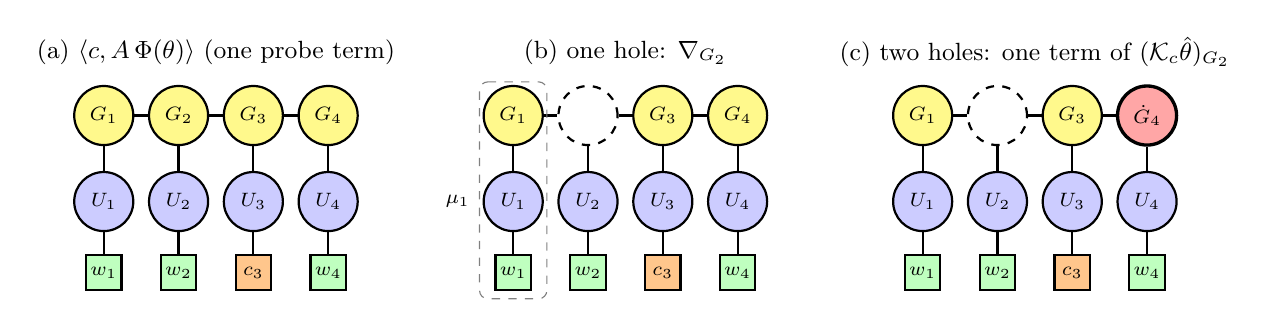
\begin{tikzpicture}[x=9.5mm,y=9.5mm]
  % (a) the sampled network
  \begin{scope}
    \foreach \i/\n in {1/G_1,2/G_2,3/G_3,4/G_4} \node[ttc] (g\i) at (\i,0) {$\n$};
    \foreach \i/\n in {1/U_1,2/U_2,3/U_3,4/U_4} \node[tkc] (u\i) at (\i,-1.15) {$\n$};
    \node[vecn] (w1) at (1,-2.1) {$w_1$}; \node[vecn] (w2) at (2,-2.1) {$w_2$};
    \node[resn] (z3) at (3,-2.1) {$c_3$}; \node[vecn] (w4) at (4,-2.1) {$w_4$};
    \foreach \i in {1,2,3} { \pgfmathtruncatemacro\j{\i+1} \draw[bnd] (g\i)--(g\j); }
    \foreach \i in {1,2,3,4} { \draw[bnd] (g\i)--(u\i); }
    \draw[bnd] (u1)--(w1); \draw[bnd] (u2)--(w2); \draw[bnd] (u3)--(z3); \draw[bnd] (u4)--(w4);
    \node[font=\small] at (2.5,0.85) {(a) $\langle c, A\,\Phi(\theta)\rangle$ (one probe term)};
  \end{scope}
  % (b) one hole
  \begin{scope}[xshift=52mm]
    \node[ttc] (g1) at (1,0) {$G_1$}; \node[holec] (g2) at (2,0) {}; \node[ttc] (g3) at (3,0) {$G_3$};
    \node[ttc] (g4) at (4,0) {$G_4$};
    \foreach \i/\n in {1/U_1,2/U_2,3/U_3,4/U_4} \node[tkc] (u\i) at (\i,-1.15) {$\n$};
    \node[vecn] (w1) at (1,-2.1) {$w_1$}; \node[vecn] (w2) at (2,-2.1) {$w_2$};
    \node[resn] (z3) at (3,-2.1) {$c_3$}; \node[vecn] (w4) at (4,-2.1) {$w_4$};
    \draw[bnd] (g1)--(g2); \draw[bnd] (g2)--(g3); \draw[bnd] (g3)--(g4);
    \foreach \i in {1,2,3,4} { \draw[bnd] (g\i)--(u\i); }
    \draw[bnd] (u1)--(w1); \draw[bnd] (u2)--(w2); \draw[bnd] (u3)--(z3); \draw[bnd] (u4)--(w4);
    \draw[dashed,gray,rounded corners=3pt] (0.55,0.45)--(1.45,0.45)--(1.45,-2.45)--(0.55,-2.45)--cycle;
    \node[font=\scriptsize,anchor=east] at (0.55,-1.15) {$\mu_1$};
    \node[font=\small] at (2.5,0.85) {(b) one hole: $\nabla_{G_2}$};
  \end{scope}
  % (c) two holes
  \begin{scope}[xshift=104mm]
    \node[ttc] (g1) at (1,0) {$G_1$}; \node[holec] (g2) at (2,0) {}; \node[ttc] (g3) at (3,0) {$G_3$};
    \node[dotc] (g4) at (4,0) {$\dot G_4$};
    \foreach \i/\n in {1/U_1,2/U_2,3/U_3} \node[tkc] (u\i) at (\i,-1.15) {$\n$};
    \node[tkc] (u4) at (4,-1.15) {$U_4$};
    \node[vecn] (w1) at (1,-2.1) {$w_1$}; \node[vecn] (w2) at (2,-2.1) {$w_2$};
    \node[resn] (z3) at (3,-2.1) {$c_3$}; \node[vecn] (w4) at (4,-2.1) {$w_4$};
    \draw[bnd] (g1)--(g2); \draw[bnd] (g2)--(g3); \draw[bnd] (g3)--(g4);
    \foreach \i in {1,2,3,4} { \draw[bnd] (g\i)--(u\i); }
    \draw[bnd] (u1)--(w1); \draw[bnd] (u2)--(w2); \draw[bnd] (u3)--(z3); \draw[bnd] (u4)--(w4);
    \node[font=\small] at (2.5,0.85) {(c) two holes: one term of $(\K_c\hat\theta)_{G_2}$};
  \end{scope}
\end{tikzpicture}
\caption{Cores as nodes, bonds as edges (TT cores on top, Tucker factors below, sample vectors as squares).
(a) One term of $\ip{c}{A\Phi(\th)}$ for a probe: the weighted residual $c_3$ sits on the free mode.
(b) The one-hole sweep (the corewise transpose) leaves one core out: the open legs are its gradient block, here
the left environment $\mu_1$ (dashed box), the projected probe $\xi_2=U_2w_2$ and a right environment.
(c) The two-hole sweep leaves one core out \emph{and} replaces another by its direction ($\dot G_4$, red); summing
over the replaced core $b\neq a$ gives block $a$ of $\K_c\thh$ (eq.~\eqref{eq:Kdef}).}
\label{fig:holes}
\end{figure}

% =====================================================================================================
\section{The exact Riemannian Hessian}
\label{sec:hessian}

\subsection{The Weingarten term as a second derivative of \texorpdfstring{$\Phi$}{Phi}}

\begin{proposition}[the curvature term, \cite{AMT13}]
\label{prop:weingarten}
Let $\zeta,\zeta'\in T_X\M$ and let $\thh,\thh'$ be any raw directions with $D\Phi(\th)[\thh]=\zeta$,
$D\Phi(\th)[\thh']=\zeta'$. Then
\begin{equation}
  \label{eq:hess}
  \ip{\Hess f(X)[\zeta]}{\zeta'} = \ip{\omega\odot A\zeta}{\omega\odot A\zeta'}
     + \ip{N}{D^2\Phi(\th)[\thh,\thh']},
\end{equation}
and the second term does not depend on the choice of lifts.
\end{proposition}

\begin{proof}
For an embedded submanifold, $\Hess f(X)[\zeta]=P_X\nabla^2 f\,\zeta+\W_X(\zeta,N)$ with the Weingarten map
$\W_X(\zeta,N)=P_X\,(D_\zeta P)\,N$, and $\ip{\W_X(\zeta,N)}{\zeta'}=\ip{N}{\mathrm{II}_X(\zeta,\zeta')}$
\cite{AMT13}. The curve $s\mapsto\Phi(\th+s\thh+s'\thh')$ lies in $\M$; by the Gauss formula the normal part of
its mixed second derivative is $\mathrm{II}_X(\zeta,\zeta')$, so
$\ip{N}{D^2\Phi[\thh,\thh']}=\ip{N}{\mathrm{II}_X(\zeta,\zeta')}$, which depends on $\zeta,\zeta'$ only. The first
term is $\ip{\zeta'}{P_XA^\T\omega^2A\zeta}=\ip{\omega A\zeta}{\omega A\zeta'}$ since $\zeta'$ is tangent.
\end{proof}

Lift independence is visible directly for the gauge directions: a \emph{vertical} direction $\thh_v=V\th$, with $V$ a linear generator of
the gauge action ($D\Phi(\th)[V\th]=0$ for \emph{every} $\th$), satisfies, after differentiating that identity along
$\thh'$, $D^2\Phi[\thh_v,\thh']=-D\Phi[V\thh']\in T_X\M$, which $N$ annihilates. (At a slack frame
$\ker D\Phi(\th)$ is larger than the gauge orbit's tangent; Proposition~\ref{prop:weingarten} covers every lift.) No derivative of the frame (no SVD perturbation) enters --- this is the reason for the route
(the archived design plan's ``route (b)''; contrast Novikov, Rakhuba \&\ Oseledets \cite{NRO22}, whose
stop-gradient on the projector gives exactly the Gauss--Newton term).

\paragraph{Core-coordinate second derivatives.} For a fixed ambient $Z$ define
\begin{equation}
  \label{eq:Kdef}
  \K_Z\,\thh \;=\; \frac{d}{ds}\nabla_\th\ip{Z}{\Phi(\th+s\thh)}\Big|_{s=0},
  \qquad \ip{\thh'}{\K_Z\thh}=\ip{Z}{D^2\Phi(\th)[\thh,\thh']},
\end{equation}
symmetric and linear in $Z$. Block $a$ of $\K_Z\thh$ is
$\sum_{b\neq a}\nabla_{\th_a}\ip{Z}{\Phi(\th;\,b\leftarrow\thh_b)}$ --- one core out, one replaced
(Figure~\ref{fig:holes}c). Two instances are needed, and $\ip{N}{D^2\Phi}$ is their difference:
\begin{itemize}
  \item $Z=\nabla f=A^\T(\omega^2\odot r)$: $\nabla_\th\ip{Z}{\Phi(\th)}$ is the kind's \emph{corewise transpose}
    at the weighted residual $c=\omega^2\odot r$, so $\K_{A^\T\omega^2r}$ is its directional derivative, the
    \emph{two-hole sweep} of Section~\ref{sec:twohole} (\code{SamplingKind.corewise_hessian});
  \item $Z=\grad f$, a doubled-rank T3 (\code{tv_to_t3}$(\text{frame},g)$; T4S App.~A.3.1, (50)--(53)): the
    T3-to-T3 two-hole of Section~\ref{sec:t3t3} (\code{ManifoldGeometryOps.tangential_curvature}).
\end{itemize}
Writing $\K_N := \K_{A^\T\omega^2r}-\K_{\grad f}$, \eqref{eq:hess} reads
$\ip{\Hess f[\zeta]}{\zeta'}=\ip{\omega A\zeta}{\omega A\zeta'}+\ip{\thh'}{\K_N\thh}$.

\subsection{The Lagrangian form, and the two levels}

Equivalently, \eqref{eq:hess} is the core-coordinate Hessian of the \emph{Lagrangian}
\begin{equation}
  \label{eq:lagrangian}
  \Lambda(\th) = f(\Phi(\th)) - \ip{\grad f(X)}{\Phi(\th)}, \qquad
  \nabla_\th\Lambda = D\Phi^\T N = 0,\qquad
  \nabla^2_\th\Lambda = D\Phi^\T\,\Hess f(X)\,D\Phi,
\end{equation}
($\grad f(X)$ frozen). $\th$ is a critical point of $\Lambda$, so its Hessian is tensorial and the vertical
directions lie in its null space. Dropping the gradient term gives the plain core Hessian of $f\circ\Phi$:
\begin{center}
\small
\begin{tabular}{@{}lll@{}}
\toprule
level & operator on gauged coordinates & exact when \\
\midrule
0, Gauss--Newton & $\Pi\Jac^\T\omega^2\Jac\Pi$ & $N=0$ \\
1, core-space Newton & $\Pi\Jac^\T\omega^2\Jac\Pi+\Pi\Lift^\T\K_{A^\T\omega^2r}\Lift\Pi
   =\Pi\Lift^\T\nabla^2_\th(f\circ\Phi)\Lift\Pi$ & $\grad f=0$ \\
2, Riemannian Newton (shipped) & level 1 $-\;\Pi\Lift^\T\K_{\grad f}\Lift\Pi=\Pi\Lift^\T\nabla^2_\th\Lambda\Lift\Pi$
   & always \\
\bottomrule
\end{tabular}
\end{center}
($\Lift$ is the undamped lift of Section~\ref{sec:lift}; with a damping $\eps>0$ the Gauss--Newton term stays
exact and only the curvature term is filtered.) Level 1 is the second derivative of $f$ along the parametrization
chart $t\mapsto\Phi(\th+t\Lift p)$, which is only a first-order retraction; it differs from level 2 by
$\ip{\grad f}{P_XD^2\Phi[\cdot,\cdot]}=O(\|\grad f\|)$ and depends on the lift. Level 2 is what the library ships;
its correction $\K_{\grad f}$ is independent of the number of samples.

\paragraph{The retraction is second order (measured).} The model is consistent with the step the optimizer takes
because the T3-SVD retraction (\code{tv_retract}, the implicit T3-SVD of T4S Algorithm~10, App.~A.2) is
\emph{second order}: $\frac{d^2}{dt^2}f(R_X(t\zeta))|_0=\ip{\Hess f[\zeta]}{\zeta}$. The archived design note
argues it as a composition of exact metric projections onto smooth bounded-rank varieties (each truncation is
Eckart--Young for one unfolding behind an isometric environment; cf.\ \cite{AM12}); the library does not rely on
the argument but on measurement: $252.85288420$ vs $252.85288182$ (design-plan check F6), the
\code{Problem.local_model} doctest, the per-kind test within $10^{-3}$ of the curvature term itself, the shared
retraction's finite-difference ratios $4.0$ and $4.25$ ($O(h^2)$, F14), and $3.7\times10^{-6}$ here (check C8a,
Richardson). The second order presumes a minimal, numerically full-rank frame (\code{retract} preserves the frame
ranks only there --- a caveat, not a precondition).

\subsection{The lift}
\label{sec:lift}

\paragraph{Frame factors.} The frame construction produces, and discards, two small matrices per mode; the library
recomputes them by contraction only (\code{fv_center_factors}; I-1: never stored on the frame, never re-SVD'd):
\begin{equation}
  \label{eq:factors}
  T_i = \ip{P_{>i}}{Q_{>i}}\in\R^{r^L_i\times r^R_i}\ (i<d),\qquad
  H_i = P_i\times_3T_i\ (H_d=P_d),\qquad
  S_i^\T = \ip{O_i}{H_i}_{\{1,3\}}\in\R^{n^D_i\times n_i},
\end{equation}
($T_i$ contracts the cores right of bond $i$: the right-to-left zipper of the left chain against the right chain,
\code{tt_zipper_right_to_left}). Then $H_i=O_i\times_2S_i^\T$, the centers are the point's own core with the
orthogonality center at $i$ ($X=P_{<i}H_iQ_{>i}\times U$), $P_{>i}=T_i\,Q_{>i}$ (the left-canonical tail is
$T_i$ times the right-orthogonal one), $\sigma(S_i)$ is the mode-$i$ Tucker spectrum, $\sigma(T_i)$ the bond-$i$
TT spectrum, and $\|X\|^2_{HS}=\|S_1^\T\|_F^2$ (checks C1a--e).

\begin{proposition}[the lift]
\label{prop:lift}
Define $\Lift v=\thh=(\dot U_i,\dot G_i)$, a variation of the base point $\th=(U,P)$, by
\begin{equation}
  \label{eq:lift}
  \dot U_i = (S_i^\T)^{+}\,\delta U_i,\qquad
  \dot G_i = \delta G_i\times_3 T_i^{+}\ (i<d),\qquad \dot G_d=\delta G_d .
\end{equation}
If every $S_i^\T$ has full row rank and every $T_i$ full column rank, then $D\Phi(\th)[\Lift v]=\Emap v$ for
\emph{all} coordinates $v$, gauged or not.
\end{proposition}

\begin{proof}
TT slot: $P_{<i}\dot G_iP_{>i}=P_{<i}\,(\dot G_iT_i)\,Q_{>i}=P_{<i}\,\delta G_i T_i^+T_i\,Q_{>i}$, and $T_i^+T_i=I$
for full column rank. Tucker slot: replacing $U_i$ by $\dot U_i$ in $X=P_{<i}H_iQ_{>i}\times U$ gives
$P_{<i}(H_i\times_2\dot U_i)Q_{>i}=P_{<i}\big(O_i\times_2(S_i^\T\dot U_i)\big)Q_{>i}$, and $S_i^\T(S_i^\T)^+=I$
for full row rank. Compare \eqref{eq:E}.
\end{proof}

Every frame \code{t3_orthogonal_representations} builds meets the hypothesis when it is numerically full rank,
minimal or not: Tucker slack makes $S_i^\T$ wide and TT slack makes $T_i$ tall, and on both the pseudo-inverse is
an exact one-sided inverse (checks C2a--c, F2/F3). Only a hand-built frame with a wide $T_i$ would give a
least-squares lift (a caveat the library never reaches). Figure~\ref{fig:lift} draws the two slots.

\begin{figure}[t]
\centering
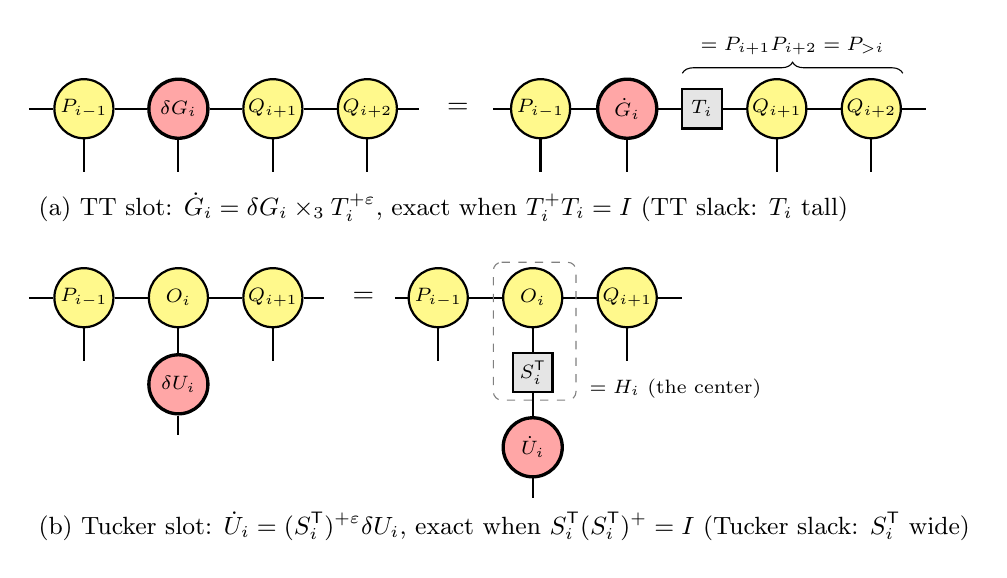
\begin{tikzpicture}[x=10mm,y=10mm]
  % (a) TT slot
  \begin{scope}
    \node[ttc] (a1) at (0,0) {$P_{i-1}$}; \node[dotc] (a2) at (1.2,0) {$\delta G_i$};
    \node[ttc] (a3) at (2.4,0) {$Q_{i+1}$}; \node[ttc] (a4) at (3.6,0) {$Q_{i+2}$};
    \draw[bnd] (-0.7,0)--(a1)--(a2)--(a3)--(a4)--(4.25,0);
    \foreach \x in {0,1.2,2.4,3.6} \draw[bnd] (\x,-0.38)--(\x,-0.8);
    \node at (4.75,0) {$=$};
    \node[ttc] (b1) at (5.8,0) {$P_{i-1}$}; \node[dotc] (b2) at (6.9,0) {$\dot G_i$};
    \node[matn] (bt) at (7.85,0) {$T_i$};
    \node[ttc] (b3) at (8.8,0) {$Q_{i+1}$}; \node[ttc] (b4) at (10.0,0) {$Q_{i+2}$};
    \draw[bnd] (5.2,0)--(b1)--(b2)--(bt)--(b3)--(b4)--(10.7,0);
    \foreach \x in {5.8,6.9,8.8,10.0} \draw[bnd] (\x,-0.38)--(\x,-0.8);
    \draw[decorate,decoration={brace,amplitude=4pt}] (7.6,0.45)--(10.4,0.45)
      node[midway,above=3pt,font=\scriptsize]{$=P_{i+1}P_{i+2}=P_{>i}$};
    \node[font=\small,anchor=west] at (-0.7,-1.25) {(a) TT slot: $\dot G_i=\delta G_i\times_3T_i^{+\eps}$, exact when $T_i^+T_i=I$ (TT slack: $T_i$ tall)};
  \end{scope}
  % (b) Tucker slot
  \begin{scope}[yshift=-24mm]
    \node[ttc] (c1) at (0,0) {$P_{i-1}$}; \node[ttc] (c2) at (1.2,0) {$O_i$}; \node[ttc] (c3) at (2.4,0) {$Q_{i+1}$};
    \node[dotc] (cu) at (1.2,-1.1) {$\delta U_i$};
    \draw[bnd] (-0.7,0)--(c1)--(c2)--(c3)--(3.05,0); \draw[bnd] (c2)--(cu)--(1.2,-1.75);
    \draw[bnd] (0,-0.38)--(0,-0.8); \draw[bnd] (2.4,-0.38)--(2.4,-0.8);
    \node at (3.55,0) {$=$};
    \node[ttc] (d1) at (4.5,0) {$P_{i-1}$}; \node[ttc] (d2) at (5.7,0) {$O_i$}; \node[ttc] (d3) at (6.9,0) {$Q_{i+1}$};
    \node[matn] (ds) at (5.7,-0.95) {$S_i^\T$};
    \node[dotc] (du) at (5.7,-1.9) {$\dot U_i$};
    \draw[bnd] (3.95,0)--(d1)--(d2)--(d3)--(7.6,0); \draw[bnd] (d2)--(ds)--(du)--(5.7,-2.55);
    \draw[bnd] (4.5,-0.38)--(4.5,-0.8); \draw[bnd] (6.9,-0.38)--(6.9,-0.8);
    \draw[dashed,rounded corners=3pt,gray] (5.2,0.45)--(6.25,0.45)--(6.25,-1.3)--(5.2,-1.3)--cycle;
    \node[font=\scriptsize,anchor=west] at (6.3,-1.15) {$=H_i$ (the center)};
    \node[font=\small,anchor=west] at (-0.7,-2.9) {(b) Tucker slot: $\dot U_i=(S_i^\T)^{+\eps}\delta U_i$, exact when $S_i^\T(S_i^\T)^+=I$ (Tucker slack: $S_i^\T$ wide)};
  \end{scope}
\end{tikzpicture}
\caption{The lift, slot by slot (red: the variation). (a) The frame's TT slot $P_{<i}\,\delta G_i\,Q_{>i}$ equals the
raw slot $P_{<i}\,\dot G_i\,P_{>i}$ because the left-canonical tail is $P_{>i}=T_iQ_{>i}$. (b) The frame's Tucker
slot pairs $\delta U_i$ with the orthonormal $O_i$; the raw slot pairs $\dot U_i$ with the center
$H_i=O_i\times_2S_i^\T$. The pseudo-inverses are the only place an inverse singular value enters the Hessian.}
\label{fig:lift}
\end{figure}

\paragraph{Damping.} The lift is the only place $1/\sigma$ appears (the TT part is the analogue of Psenka \&\ Boumal's
$R_k^{-1}$ \cite{PB20}), so it is damped by the Tikhonov filter
\begin{equation}
  \label{eq:filter}
  f_\eps(\sigma)=\frac{\sigma}{\sigma^2+\eps^2}\ \ (0\text{ for }\sigma\le\mathrm{rcond}\cdot\sigma_1),\qquad
  M^{+\eps}=V f_\eps(\Sigma)U^\T=(M^\T M+\eps^2I)^{-1}M^\T,
\end{equation}
with the absolute damping $\eps=\texttt{curvature\_damping}\cdot\|X\|_{HS}$
(\code{filtered_reciprocal}, \code{damped_pseudo_inverse} in \code{backend/linalg.py};
$\|X\|_{HS}=\|S_1^\T\|_F$; default \code{DEFAULT_CURVATURE_DAMPING} $=10^{-6}$ in \code{backend/geometry.py}).
$f_\eps\le1/(2\eps)$ (check C4a), $f_\eps\approx1/\sigma$ for $\sigma\gg\eps$, $\approx\sigma/\eps^2$ below; the
relative clip (default dtype-$\eps$ times the larger dimension, \code{numpy.linalg.pinv}'s) maps roundoff
singular values to exactly $0$, which is why a zero-padded rank-continuation restart (new singular values
$\sim10^{-17}$) needs no special case: there the lift satisfies $D\Phi[\Lift v]=\Emap(Q_{\mathrm c}v)$ with $Q_{\mathrm c}$ the
projection off the clipped directions, the Hessian is Gauss--Newton in them, and the trust region bounds the step.
The last TT slot passes through undamped. The damping is a \emph{solver option}, never a geometry field: it reaches
the computation only through the traced leaf \code{LiftFactors.eps}, so a new damping never recompiles (I-22).

\paragraph{The transpose.} $\Lift^\T y$ maps raw core variations $y=(Y^U_i,Y^G_i)$ to \emph{ungauged}
coordinates, $\delta U_i=((S_i^\T)^{+\eps})^\T Y^U_i$, $\delta G_i=Y^G_i\times_3(T_i^{+\eps})^\T$,
$\delta G_d=Y^G_d$, with the \emph{same} factors, so $\Lift_\eps^\T\K\Lift_\eps$ is symmetric for every $\eps$
(check C3). The Hessian applies $\Pi$ outside.

\begin{algorithm}[t]
\caption{The lift $\thh=\Lift_\eps v$ and its adjoint $\Lift_\eps^\T$ (per-frame factors once, per matvec two
contractions per mode)}
\label{alg:lift}
\begin{algorithmic}[1]
\Require orthogonal frame $(U,O,P,Q)$; relative damping $c\ge0$; coordinates $v=(\delta U_i,\delta G_i)$ (stack $\mathtt{K+C}$)
\Ensure raw directions $\thh=(\dot U_i,\dot G_i)$ of $\th=(U,P)$
\State $T_i\gets\ip{P_{>i}}{Q_{>i}}$ (zipper);\ $H_i\gets P_i\times_3T_i$;\ $S_i^\T\gets\ip{O_i}{H_i}_{\{1,3\}}$
   \Comment{\code{fv_center_factors}}
\State $\eps\gets c\,\|S_1^\T\|_F$;\ $(S_i^\T)^{+\eps},\ T_i^{+\eps}\gets$ one thin SVD each, filter \eqref{eq:filter}
   \Comment{\code{fv_lift_factors}}
\For{$i=1,\dots,d$} \Comment{\code{tv_corewise_lift}}
  \State $\dot U_i\gets(S_i^\T)^{+\eps}\,\delta U_i$ \Comment{\texttt{'Cux,KCxn->KCun'}}
  \State $\dot G_i\gets\delta G_i\times_3T_i^{+\eps}$ if $i<d$, else $\dot G_d\gets\delta G_d$ \Comment{\texttt{'KCaib,Cbc->KCaic'}}
\EndFor
\State adjoint: $\delta U_i\gets((S_i^\T)^{+\eps})^\T Y^U_i$,\ $\delta G_i\gets Y^G_i\times_3(T_i^{+\eps})^\T$
   \Comment{\code{tv_corewise_lift_transpose}}
\Impl{\code{fv_operations.fv_center_factors}, \code{fv_operations.fv_lift_factors} (\code{LiftFactors}),
\code{linalg.damped_pseudo_inverse}, \code{linalg.filtered_reciprocal}, \code{tv_operations.tv_corewise_lift[_transpose]};
uniform: \code{ufv_operations.ufv_lift_factors}, \code{utv_operations.utv_corewise_lift[_transpose]}.}
\end{algorithmic}
\end{algorithm}

\subsection{The Newton system}
\label{sec:system}

In gauged coordinates, with the identity regularizer $\rho(X)=\frac\lambda2\|X\|^2$ (whose Hessian $\lambda\Pi$ is
already exact: $X$ lies in its own tangent space),
\begin{equation}
  \label{eq:newton}
  \boxed{\;\Hop p \;=\; \Pi\Jac^\T\omega^2\Jac\Pi p \;+\; \Pi\Lift^\T\big(\K_{A^\T\omega^2 r}-\K_{\grad f}\big)\Lift\Pi p
  \;+\;\lambda\Pi p\;}
\end{equation}
(\code{LocalModel.hvp}); the curvature uses the \emph{misfit} gradient only. On the corewise geometry the exact
Hessian is the plain Hessian of $f\circ\Phi$, $\Jac_c^\T\omega^2\Jac_c+\K_{A^\T\omega^2r}$: no lift, no gradient
term (the corewise geometry's \code{lift} is the identity, \code{tangential_curvature} returns \code{None}). The
model does \emph{one} misfit transpose per Newton step: \code{Problem.local_model(hessian='exact')} computes
$g=\Pi\Jac^\T\omega^2r$ once into \code{CurvatureState.misfit_gradient}, read by both \code{LocalModel.gradient}
(bit-identical to Gauss--Newton's, check C14c) and \code{curvature_precompute}. The per-step overhead is the
doubled-rank $Z=\grad f$, one T3-to-T3 sweep and $2d-1$ small SVDs.

\begin{algorithm}[t]
\caption{The exact Hessian-vector product \eqref{eq:newton}}
\label{alg:hvp}
\begin{algorithmic}[1]
\Require local model at $X$: frame, sampling sweep, residual $r$, curvature data
  $(\Lift\text{ factors}, Z=\grad f, Z\text{-sweep})$; direction $p$ (stack $\mathtt{K+C}$)
\Ensure $\Hop p$
\State $p\gets\Pi p$;\quad $z\gets\Jac p$ \Comment{\code{SamplingKind.forward}}
\State $\thh\gets\Lift p$ \Comment{\code{geom.lift}}
\State $k\gets\K_{A^\T\omega^2r}\,\thh$ \Comment{two-hole, \code{kind.corewise_hessian} (Alg.~\ref{alg:driver})}
\State $k\gets k-\K_{\grad f}\,\thh$ \Comment{T3--T3 two-hole, \code{geom.tangential_curvature} (Alg.~\ref{alg:t3t3})}
\State $y\gets\Lift^\T k$ \Comment{\code{geom.lift_transpose}, ungauged}
\State \Return $\Pi\big(\Jac^\T\omega^2 z+y\big)+\lambda\Pi p$ \Comment{one projection for both terms}
\Impl{\code{optimizers.LocalModel.hvp}, \code{LocalModel._curvature_block}, \code{curvature_hvp},
\code{quadratic} $=$ \code{gn_quadratic} $+$ \code{curvature_quadratic}; per frame:
\code{Problem.local_model}, \code{CurvatureState}, \code{ManifoldGeometryOps.curvature_precompute}
(\code{ManifoldCurvatureData}: \code{fv_lift_factors}, \code{tv_to_t3}, \code{t3_precompute_inner_product_sweep},
\code{_lift_sigma_min}); uniform: \code{UniformManifoldGeometryOps.curvature_precompute}.}
\end{algorithmic}
\end{algorithm}

\paragraph{Where the term vanishes.} At a slot of \emph{maximal} rank (a Tucker rank equal to the mode size, a TT
rank equal to the product of its neighbours) the representable set is locally open in that slot's directions and
$N$ has no component there; at $d=1$ every slot is maximal and $N\equiv0$. The formula needs no special case
(the filtered pseudo-inverses and the two-hole sum give $\Lift^\T\K_N\Lift=0$); the manifold geometry's
\code{curvature_precompute} returns \code{None} at $d=1$ purely to skip the work.

% =====================================================================================================
\section{The two-hole sweep}
\label{sec:twohole}

\subsection{The one-hole sweep it differentiates}

At the \emph{corewise frame} $(U,G,G,G)$ of raw cores $\th=(U,G)$ (\code{t3_corewise_frame}) the tangent
transpose of T4S Algorithm~8 is the core gradient $\nabla_\th\ip{c}{A\Phi(\th)}$ (T4S \S6.3, the corewise
substitution $P,Q,O\to G$; \code{t3_probe_corewise_transpose}). With edge variables on bonds $0,\dots,d$ (core $i$
joins bonds $i-1$ and $i$; $G_i(x)$ contracts the middle index of $G_i$ with $x$):
\begin{align}
  \label{eq:fwd}
  &\xi_i=U_iw_i,\quad \mu_i=\mu_{i-1}G_i(\xi_i),\ \mu_0=1,\quad \nu_{i-1}=G_i(\xi_i)\nu_i,\ \nu_d=1,\quad
   \eta_i=\mu_{i-1}G_i\nu_i, \\
  \label{eq:adj}
  &\ddet_i=U_ic_i,\quad \tilde\tau_i=\tilde\tau_{i-1}G_i(\xi_i)+\mu_{i-1}G_i(\ddet_i),\ \tilde\tau_0=0,\quad
   \tilde\sigma_{i-1}=G_i(\xi_i)\tilde\sigma_i+G_i(\ddet_i)\nu_i,\ \tilde\sigma_d=0, \\
  \label{eq:dxt}
  &\dxt_i=\tilde\tau_{i-1}G_i\nu_i+\mu_{i-1}G_i\tilde\sigma_i, \\
  \label{eq:asm}
  &\delta\tilde U_i=\textstyle\sum_{\mathtt W}\big(\eta_i\otimes c_i+\dxt_i\otimes w_i\big),\qquad
   \delta\tilde G_i=\sum_{\mathtt W}\big(\mu_{i-1}\otimes\xi_i\otimes\tilde\sigma_i
   +\tilde\tau_{i-1}\otimes\xi_i\otimes\nu_i+\mu_{i-1}\otimes\ddet_i\otimes\nu_i\big).
\end{align}
The TT gradient has three trilinear groups (the core-adjoints of the forward $\sigma$, $\tau$, $\delta\eta$ of
T4S Algorithm~7); the Tucker gradient has one internal edge. Apply and entries (\code{t3_apply_corewise_transpose})
are the all-modes case: a scalar residual $c$ seeds one propagation sweep
$\hat\sigma_{i-1}=G_i(\xi_i)\hat\sigma_i$, $\hat\sigma_d=c$, and $\delta\tilde G_i=\sum_{\mathtt W}\mu_{i-1}\otimes
\xi_i\otimes\hat\sigma_i$, $\delta\tilde U_i=\sum_{\mathtt W}\delta\hat\xi_i\otimes w_i$ with
$\delta\hat\xi_i=\mu_{i-1}G_i\hat\sigma_i$.

\begin{algorithm}[t]
\caption{The one-hole sweep (reference): the corewise probe transpose $\nabla_\th\ip{c}{A\Phi(\th)}$}
\label{alg:onehole}
\begin{algorithmic}[1]
\Require $\th=(U_i,G_i)$; probe vectors $w_i$ (stack $\mathtt W$); weighted residuals $c_i=\omega_i^2\odot r_i$
\Ensure $(\delta\tilde U_i,\delta\tilde G_i)$, $\mathtt W$ summed
\State $\xi_i,\mu_i,\nu_i,\eta_i$ by \eqref{eq:fwd} \Comment{frame sweep (T4S Alg.~5); \code{tv_precompute_probe_frame_sweep}}
\State $\ddet_i\gets U_ic_i$ \Comment{\code{compute_deta_tilde}}
\For{$i=1,\dots,d$} $\tilde\tau_i\gets\tilde\tau_{i-1}G_i(\xi_i)+\mu_{i-1}G_i(\ddet_i)$ \Comment{\code{compute_tau_tilde}}
\EndFor
\For{$i=d,\dots,1$} $\tilde\sigma_{i-1}\gets G_i(\xi_i)\tilde\sigma_i+G_i(\ddet_i)\nu_i$ \Comment{\code{compute_sigma_tilde}}
\EndFor
\State $\dxt_i\gets\tilde\tau_{i-1}G_i\nu_i+\mu_{i-1}G_i\tilde\sigma_i$ \Comment{\code{compute_dxi_tilde}}
\State $\delta\tilde U_i,\ \delta\tilde G_i$ by \eqref{eq:asm} \Comment{\code{assemble_tucker_variations}, \code{assemble_tt_variations}}
\Impl{\code{probing.t3_probe_corewise_transpose} = \code{probing.tv_probe_transpose} at \code{fv_conversions.t3_corewise_frame}
(T4S \S6.2.3, Algorithm~8; \S6.3). Jets: \code{sampling_derivatives.t3_probe_corewise_derivatives_transpose},
\code{tv_probe_transpose_derivatives_from_sweep}.}
\end{algorithmic}
\end{algorithm}

\subsection{Two holes: the product rule of the one-hole sweep}

Every quantity in \eqref{eq:fwd}--\eqref{eq:asm} is multilinear in the cores and the sample vectors. For fixed $c$
the one-hole output is $\nabla_\th\ip{c}{A\Phi(\th)}$, so by \eqref{eq:Kdef} $\K_c\thh$ is its directional
derivative along $\thh=(\dot U_i,\dot G_i)$, i.e.\ the \emph{product rule} applied to every line of
Algorithm~\ref{alg:onehole}: each edge variable gains a \emph{dotted} companion carrying the tangent stack
$\mathtt K$ (``exactly one core replaced''), while $c$, $w$ and the undotted state carry $\mathtt{W+C}$ only.
Two observations make this cheap:

\begin{enumerate}
\item \textbf{The dotted forward is the Gauss--Newton tangent forward at the corewise frame.} Differentiating
  \eqref{eq:fwd} gives
  $\dot\xi_i=\dot U_iw_i$,\
  $\dot\mu_i=\dot\mu_{i-1}G_i(\xi_i)+\mu_{i-1}\dot G_i(\xi_i)+\mu_{i-1}G_i(\dot\xi_i)$,\
  $\dot\nu_{i-1}=G_i(\xi_i)\dot\nu_i+\dot G_i(\xi_i)\nu_i+G_i(\dot\xi_i)\nu_i$,\
  $\dot\eta_i=\dot\mu_{i-1}G_i\nu_i+\mu_{i-1}\dot G_i\nu_i+\mu_{i-1}G_i\dot\nu_i$
  --- exactly T4S Algorithm~7 ($\sigma,\tau,\delta\eta$) with $Q=O=P=G$ and variation $(\dot U,\dot G)$. The
  library calls its own GN tangent forward (\code{compute_sigma}, \code{compute_tau}, \code{compute_deta};
  jets: \code{compute_sigma_jets}, \code{compute_tau_jets}, \code{compute_deta_jets}).
\item \textbf{No undotted $\eta$ or $\dxt$ at the corewise frame is needed.} With $c$ and $w$ fixed,
  $\frac{d}{ds}\delta\tilde U_i=\sum_{\mathtt W}(\dot\eta_i\otimes c_i+\dot{\dxt}_i\otimes w_i)$, and $\delta\tilde G_i$
  involves neither. The default is \emph{recompute} (I-11): $\xi,\mu$ are reused from the model's sweep (identical at
  the manifold frame $(U,O,P,Q)$ and the corewise frame $(U,P,P,P)$ of the base point), $\nu$ is re-swept through
  $G$ (1--3\% of the two-hole), and nothing else is stored. (At the manifold frame the corewise state is a cheap
  $T$/$S$ transform of the manifold one, $\nu_c=T\nu$, $\eta_c=S\eta$ --- F16 --- which a deferred ``store''
  variant would use.)
\end{enumerate}

\paragraph{The block-sum oracle.} Since $D\Phi(\th)[\thh]=\Phi(Y)$ for the doubled-rank T3 $Y$ that
\code{tv_to_t3} builds from $\thh$ at \code{t3_corewise_frame}$(\th)$, whose blocks are cores of $\th$, of $\thh$ or
zero, and $Y$ is affine in $\th$ (its $\thh$ blocks fixed),
\begin{equation}
  \label{eq:blocksum}
  \K_c\thh = B^\T\,\nabla_Y\ip{c}{A\Phi(Y)},
\end{equation}
$B^\T$ summing the gradient blocks where $\th$'s cores sit. This one-hole-only identity (check C9b, $3.4\times10^{-16}$)
is the reference every two-hole is tested against (\code{tests/backend/_curvature_oracles.py}); the others are
\code{jax.jvp} of the shipped one-hole and, for the whole Hessian, a dense extrinsic Weingarten oracle
(\code{tests/oracle_sweeps/sweep_exact.py}).

\subsection{Two-index jets and the recurrence-only rule}
\label{sec:jets}

For the derivative kinds every edge variable is a jet $x=(x^{(0)},\dots,x^{(m)})$ along the sample direction
$w+sp$, and the core direction is a \emph{second, independent} index truncated at first order. Leibniz in the core
index needs no binomials, $\frac{d}{ds}(fgh)=\dot fgh+f\dot gh+fg\dot h$, so each three-factor jet product of the GN
kernels spawns three dotted products with the same order wiring. Layout: \emph{companion arrays} (I-10) ---
undotted jets $(m{+}1,)+\mathtt{W+C}+(\cdot)$, dotted ones $(m{+}1,)+\mathtt{W+K+C}+(\cdot)$ --- never a stacked
length-2 axis, which would broadcast every undotted jet over $\mathtt K$.

Write the down-shift $(\Dsh x)^{(t)}=t\,x^{(t-1)}$ and its adjoint, the up-shift $(\Ush x)^{(s)}=(s+1)\,x^{(s+1)}$
($x^{(m+1)}=0$), so that $\Dsh^r x=r!\binom{t}{r}x^{(t-r)}$ and $(\Ush^rx)^{(s)}=r!\binom{r+s}{r}x^{(r+s)}$
(\code{_shift_down}, \code{_shift_up}). The input jets are affine, $\xi_i=(U_iw_i,U_ip_i)$,
$\dot\xi_i=(\dot U_iw_i,\dot U_ip_i)$ (\code{build_input_jets}). Every jet product is one of four forms:
\begin{align}
  \label{eq:band}
  &\text{banded (one affine factor } b\text{):} && (a\star b)^{(t)}=a^{(t)}b^{(0)}+(\Dsh a)^{(t)}b^{(1)},
     && (c\star^\T b)^{(s)}=c^{(s)}b^{(0)}+(\Ush c)^{(s)}b^{(1)},\\
  \label{eq:conv}
  &\text{full (both jets):} && (a\ast b)^{(t)}=\textstyle\sum_r\frac{a^{(r)}}{r!}(\Dsh^r b)^{(t)},
     && (a\ast^\T z)^{(s)}=\textstyle\sum_r\frac{a^{(r)}}{r!}(\Ush^r z)^{(s)},
\end{align}
the banded ones a two-term recurrence fused into one GEMM (\code{_shift_down_pair}, \code{_shift_up_pair}), the
full ones an \emph{order scan} over $r$ that carries the shifted factor, one order slice live at a time
(\code{_inverse_factorials} supplies $1/r!$). \textbf{The recurrence-only rule} (I-33): every production kernel is one
of these forms; a dense binomial tensor $\binom{t}{r}[r+s=t]$ appears only in the \code{_trs} \emph{test twins}
(\code{tests/_jet_trs_twins.py}, \code{tests/backend/_curvature_oracles.py}), which the kernels match to
$\le5.8\times10^{-16}$ over orders 0--4.

\paragraph{The jet sweeps.} With these, the GN adjoint step (\code{_adj_tilde_step}) is
$\tilde\tau_i=\tilde\tau_{i-1}\star^\T G_i(\xi_i)+\mu_{i-1}\ast^\T G_i(\ddet_i)$ --- a \emph{prop} half
(\code{_adj_prop}) and a \emph{src} half (\code{_adj_src_order_step}) --- that is,
\begin{equation}
  \label{eq:tautilde}
  \tilde\tau_i^{(s)}=\tilde\tau_{i-1}^{(s)}G_i(\xi_i^{(0)})+(s+1)\,\tilde\tau_{i-1}^{(s+1)}G_i(\xi_i^{(1)})
   +\sum_{r\ge0}\tbinom{r+s}{r}\,\mu_{i-1}^{(r)}G_i\big(\ddet_i^{(r+s)}\big),
\end{equation}
and its product rule along $(\dot G,\dot\xi,\dot\mu,\dot{\ddet})$, with $\dot{\ddet}_i=\dot U_ic_i$, is the dotted step
(\code{_adj_tilde_tangent_step}; check C10d):
\begin{equation}
  \label{eq:tautildedot}
  \dot{\tilde\tau}_i=\underbrace{\dot{\tilde\tau}_{i-1}\star^\T G_i(\xi_i)
     +\tilde\tau_{i-1}\star^\T\big(\dot G_i(\xi_i)+G_i(\dot\xi_i)\big)}_{\text{prop: \code{_adj_prop_tangent}, two GEMMs}}
   +\underbrace{\big(\dot\mu_{i-1}G_i+\mu_{i-1}\dot G_i\big)\ast^\T\ddet_i+\mu_{i-1}G_i\ast^\T\dot{\ddet}_i}
     _{\text{src: \code{_adj_tangent_src_order_step}, one scan over }r},
\end{equation}
the six dotted terms (K on the carry, the core, $\xi$; on the edge, the core, $\ddet$) paired by shared factor; the
src scan's live slice is $\mathtt W\mathtt K r^2$. $\dot{\tilde\sigma}$ is the mirror (\code{tt_reverse}). Since
$\dxt$ is the adjoint of the \emph{affine} $\delta\xi$, only its rows $u\in\{0,1\}$ are read (the Tucker assembly
pairs them with $(w,p)$), and only those are formed: with $[\Ush^0x]=x$, $[\Ush^1x]=\Ush x$,
\begin{equation}
  \label{eq:dxitilde}
  \dxt_i^{(u)}=\sum_j\mu_{i-1}^{(j)}G_i\,[\Ush^u\tilde\sigma_i]^{(j)}+[\Ush^u\tilde\tau_{i-1}]^{(j)}G_i\,\nu_i^{(j)},
  \qquad u\in\{0,1\},
\end{equation}
an order scan over $j$ (\code{compute_dxi_tilde_jets}); its dot has the six terms
$d(\mu G)[\Ush^u\tilde\sigma]+\mu G[\Ush^u\dot{\tilde\sigma}]+[\Ush^u\dot{\tilde\tau}]G\nu+[\Ush^u\tilde\tau]d(G\nu)$,
$d(\mu G)=\dot\mu G+\mu\dot G$, $d(G\nu)=\dot G\nu+G\dot\nu$ (\code{_dxi_tilde_tangent_order_step}; check C10e).

\begin{algorithm}[t]
\caption{Two-hole, forward half: the dotted forward jets along $\thh=(\dot U,\dot G)$}
\label{alg:fwd}
\begin{algorithmic}[1]
\Require $\th=(U,G)$; $\thh$ (stack $\mathtt{K+C}$); $w_i,p_i$ (stack $\mathtt W$); order $m$; model sweep $(\xi,\mu)$
\Ensure $\dot\xi_i,\dot\mu_i,\dot\nu_i,\dot\eta_i$ (orders $0..m$) and the undotted $\nu_i$
\State $\dot\xi_i\gets(\dot U_iw_i,\ \dot U_ip_i)$ \Comment{\code{build_input_jets}, \code{compute_xi}}
\State $\nu_{i-1}\gets G_i(\xi_i)\star\nu_i$ \Comment{re-swept through $G$: \code{compute_nu_jets}}
\For{$i=1,\dots,d$}
  \State $\dot\mu_i\gets\dot\mu_{i-1}\star G_i(\xi_i)+\mu_{i-1}\star\dot G_i(\xi_i)+\mu_{i-1}\star G_i(\dot\xi_i)$
  \Comment{\code{compute_sigma_jets}$(\dot G,G,G,\dots)$}
\EndFor
\For{$i=d,\dots,1$}
  \State $\dot\nu_{i-1}\gets G_i(\xi_i)\star\dot\nu_i+\dot G_i(\xi_i)\star\nu_i+G_i(\dot\xi_i)\star\nu_i$
  \Comment{\code{compute_tau_jets}}
\EndFor
\State $\dot\eta_i\gets\dot\mu_{i-1}G_i\ast\nu_i+\mu_{i-1}\dot G_i\ast\nu_i+\mu_{i-1}G_i\ast\dot\nu_i$
  \Comment{\code{compute_deta_jets} (order scan)}
\Impl{\code{sampling_derivatives}: the GN tangent forward (T4S Alg.~7 jet-ified) at $Q=O=P=G$; plain kinds
\code{probing.compute_dxi}, \code{compute_sigma}, \code{compute_tau}, \code{compute_deta}.}
\end{algorithmic}
\end{algorithm}

\begin{algorithm}[t]
\caption{Two-hole, adjoint half: the dotted adjoint sweeps}
\label{alg:adj}
\begin{algorithmic}[1]
\Require undotted $\xi,\mu,\nu$ and adjoint state $\ddet,\tilde\tau,\tilde\sigma$ at $\th$; dotted $\dot\xi,\dot\mu,\dot\nu$; residual jets $c_i$
\Ensure $\dot{\ddet}_i,\dot{\tilde\tau}_i,\dot{\tilde\sigma}_i$ and the two read rows $\dot{\dxt}_i^{(0,1)}$
\State $\dot{\ddet}_i\gets\dot U_ic_i$ \Comment{order-diagonal; \code{compute_deta_tilde_tangent_jets}}
\For{$i=1,\dots,d$} \Comment{carry $\dot{\tilde\tau}$; the undotted $\tilde\tau_{i-1}$ rides as scan data}
  \State $\dot{\tilde\tau}_i\gets$ \eqref{eq:tautildedot} \Comment{\code{compute_tau_tilde_tangent_jets}, step \code{_adj_tilde_tangent_step}}
\EndFor
\State $\dot{\tilde\sigma}\gets$ the same sweep on the reversed train \Comment{\code{compute_sigma_tilde_tangent_jets}}
\State $\dot{\dxt}_i^{(u)}\gets$ the product rule of \eqref{eq:dxitilde}, $u\in\{0,1\}$ \Comment{\code{compute_dxi_tilde_tangent_jets}}
\Impl{\code{sampling_derivatives}: \code{_adj_prop_tangent}, \code{_adj_tangent_src_order_step},
\code{_adj_tangent_sweep_scanned}, \code{_dxi_tilde_tangent_order_step}; plain probe: \code{probing.compute_deta_tilde_tangent},
\code{compute_tau_tilde_tangent} (two \code{_sigma_step} calls per core), \code{compute_sigma_tilde_tangent},
\code{compute_dxi_tilde_tangent} (two \code{compute_deta} calls).}
\end{algorithmic}
\end{algorithm}

\subsection{The assembly, factored by the product rule}
\label{sec:assembly}

The Tucker block is the derivative of a single order-sum, $\mathtt W$ summed:
\begin{equation}
  \label{eq:tuckerdot}
  (\K_c\thh)_{U_i}=\sum_{\mathtt W}\Big(\sum_t\dot\eta_i^{(t)}\otimes c_i^{(t)}+\sum_{u\in\{0,1\}}\dot{\dxt}_i^{(u)}\otimes w_i^{(u)}\Big),
  \qquad w^{(0)}=w,\ w^{(1)}=p .
\end{equation}
The TT block is the derivative of three \emph{trilinear} groups (eq.~\eqref{eq:asm}); the product rule gives nine
trilinear terms, each a $\mathtt W$-summed outer product of the size of a core. Forming each group's
\emph{pair intermediate} and its dotted twin once, before the $\mathtt W$ sum, replaces the nine large
contractions by fewer: four for the plain probe, two plus two per lag step for the jets, two (from three) for
apply / entries (below). (F33 measured the planned six-final factored jet form $1.4$--$2.0\times$ faster on that
term than the nine-term one, equal to $3\times10^{-15}$.)

\paragraph{Plain probe} (\code{probing.assemble_tt_tangent_variations}). Group by the left-bond factor:
$\delta\tilde G_i=\sum_{\mathtt W}\mu_{i-1}\cdot E_1+\tilde\tau_{i-1}\cdot E_2$ with the pairs (over the mode and
right-bond legs)
\begin{equation}
  \label{eq:pairs}
  E_1=\xi_i\otimes\tilde\sigma_i+\ddet_i\otimes\nu_i,\qquad E_2=\xi_i\otimes\nu_i,\qquad
  (\K_c\thh)_{G_i}=\sum_{\mathtt W}\dot\mu_{i-1}\cdot E_1+\mu_{i-1}\cdot\dot E_1+\dot{\tilde\tau}_{i-1}\cdot E_2+\tilde\tau_{i-1}\cdot\dot E_2,
\end{equation}
$\dot E_1=\dot\xi\otimes\tilde\sigma+\xi\otimes\dot{\tilde\sigma}+\dot{\ddet}\otimes\nu+\ddet\otimes\dot\nu$,
$\dot E_2=\dot\xi\otimes\nu+\xi\otimes\dot\nu$: four $\mathtt W$-summed finals (check C11c). Any pairing of the three
groups into two intermediates gives four; slice S3's dense form paired the $\tilde\tau$ and $\ddet$ groups through
their common $\nu$.

\paragraph{Jets} (\code{assemble_tt_tangent_variation_jets}). The $\tilde\sigma$ and $\tilde\tau$ groups share the
\emph{affine} $\xi$, so they are banded and add into one pair; the $\ddet$ group (both $\mu$, $\nu$ full) is a
\emph{lag scan}. The GN assembly (\code{assemble_tt_variation_jets}) is
\begin{equation}
  \label{eq:asmjet}
  \delta\tilde G_i=\sum_{\mathtt W}\Big(\sum_{k\in\{0,1\}}\Pi_{i,k}\otimes_2\xi_i^{(k)}
     +\sum_r\mu_{i-1}^{(r)}\otimes F_i^{(r)}\Big),\quad
  \Pi_{i,k}=\sum_r\mu_{i-1}^{(r)}\otimes[\Ush^k\tilde\sigma_i]^{(r)}+\sum_s[\Ush^k\tilde\tau_{i-1}]^{(s)}\otimes\nu_i^{(s)},
\end{equation}
with the fold $F_i^{(r)}=\sum_s\binom{r+s}{r}\ddet_i^{(r+s)}\otimes\nu_i^{(s)}=\sum_s\frac{1}{r!}(\Ush^r\ddet_i)^{(s)}\otimes\nu_i^{(s)}$
(\code{_tt_det_lag_step}, which carries $\Ush^r\ddet$). Its derivative (\code{_tt_tangent_variation_jets_step},
\code{_tt_tangent_det_lag_step}) is
\begin{equation}
  \label{eq:asmjetdot}
  (\K_c\thh)_{G_i}=\sum_{\mathtt W}\Big(\sum_k\dot\Pi_{i,k}\otimes_2\xi_i^{(k)}+\Pi_{i,k}\otimes_2\dot\xi_i^{(k)}
     +\sum_r\dot\mu_{i-1}^{(r)}\otimes F_i^{(r)}+\mu_{i-1}^{(r)}\otimes\dot F_i^{(r)}\Big),
\end{equation}
$\dot\Pi_{i,k}$ the four-term product rule of $\Pi_{i,k}$ ($\mathtt K$ on $\dot\mu$, $\dot{\tilde\sigma}$,
$\dot{\tilde\tau}$, $\dot\nu$), $\dot F^{(r)}$ the two-term one: two banded finals plus two per lag step (check
C11a: equal to the nine-term dense binomial form to $6.3\times10^{-16}$). Apply/entries have one group, so
$3\to2$ finals: $(\K_c\thh)_{G_i}=\sum_{\mathtt W}\dot\mu_{i-1}\cdot E+\mu_{i-1}\cdot\dot E$, $E=\xi_i\otimes\hat\sigma_i$.
The probe-derivative assemblies are $\mathtt W$-chunked through \code{_wchunked_sum} (per-chunk kernels
\code{_tt_tangent_chunk_summed}, \code{_tucker_tangent_chunk_summed}); the other kinds' transposes have no chunked
path, so neither do their two-holes.

\begin{figure}[t]
\centering
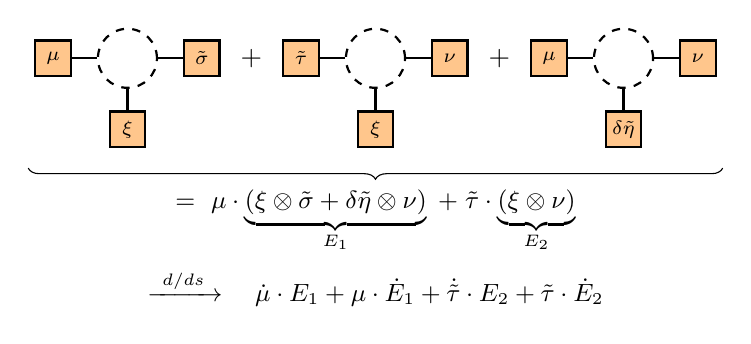
\begin{tikzpicture}[x=9mm,y=9mm]
  \newcommand{\hole}[4]{% x, left label, down label, right label
    \node[holec] (h) at (#1,0) {};
    \node[resn] (l) at ($(#1,0)+(-1.05,0)$) {$#2$};
    \node[resn] (r) at ($(#1,0)+(1.05,0)$) {$#4$};
    \node[resn] (dn) at ($(#1,0)+(0,-1.0)$) {$#3$};
    \draw[bnd] (l)--(h)--(r); \draw[bnd] (h)--(dn);}
  \hole{0}{\mu}{\xi}{\tilde\sigma}
  \node at (1.75,0) {$+$};
  \hole{3.5}{\tilde\tau}{\xi}{\nu}
  \node at (5.25,0) {$+$};
  \hole{7}{\mu}{\delta\tilde\eta}{\nu}
  \draw[decorate,decoration={brace,amplitude=4pt,mirror}] (-1.4,-1.55)--(8.4,-1.55);
  \node[font=\small] at (3.5,-2.3) {$=\ \mu\cdot\underbrace{(\xi\otimes\tilde\sigma+\delta\tilde\eta\otimes\nu)}_{E_1}
     \;+\;\tilde\tau\cdot\underbrace{(\xi\otimes\nu)}_{E_2}$};
  \node[font=\small] at (3.5,-3.25) {$\xrightarrow{\ d/ds\ }\quad \dot\mu\cdot E_1+\mu\cdot\dot E_1+\dot{\tilde\tau}\cdot E_2+\tilde\tau\cdot\dot E_2$};
\end{tikzpicture}
\caption{The TT gradient block as three trilinear outer products around the hole at core $i$ (left bond, mode
leg, right bond), and its factored derivative: the pairs $E_1,E_2$ (and their dotted twins) are formed per sample,
then four $\mathtt W$-summed contractions with the left-bond factor produce the core-sized result, instead of
nine.}
\label{fig:pairs}
\end{figure}

\begin{algorithm}[t]
\caption{The probe-derivative two-hole $\K_c\thh$ (driver)}
\label{alg:driver}
\begin{algorithmic}[1]
\Require $c_i=\omega^2\odot r_i$ (jets, $\mathtt{W+C}$); $w,p$; $\th=(U,G)$; $\thh$ ($\mathtt{K+C}$); order $m$; model sweep $(\xi,\mu)$
\Ensure $\K_c\thh$, raw core variations ($\mathtt{K+C}$, $\mathtt W$ summed)
\State undotted: $\nu$ re-swept through $G$; $\ddet=Uc$; $\tilde\tau$, $\tilde\sigma$ \Comment{GN kernels, recompute (I-11)}
\State dotted forward $\dot\xi,\dot\mu,\dot\nu,\dot\eta$ \Comment{Algorithm~\ref{alg:fwd}}
\State dotted adjoint $\dot{\ddet},\dot{\tilde\tau},\dot{\tilde\sigma},\dot{\dxt}^{(0,1)}$ \Comment{Algorithm~\ref{alg:adj}}
\State Tucker block \eqref{eq:tuckerdot}; TT block \eqref{eq:asmjetdot}, $\mathtt W$-chunked \Comment{Section~\ref{sec:assembly}}
\Impl{\code{sampling_derivatives.t3_probe_corewise_derivatives_hessian[_from_sweep]}; step 1 \code{compute_nu_jets},
\code{compute_deta_tilde_jets}, \code{compute_tau_tilde_jets}, \code{compute_sigma_tilde_jets}; step 4
\code{assemble_tucker_tangent_variation_jets}, \code{assemble_tt_tangent_variation_jets}; the other kinds:
\code{probing.t3_probe_corewise_hessian[_from_sweep]}, \code{apply.t3_apply_corewise_hessian[_from_sweep]}
(\code{_apply_corewise_hessian_adjoint}), \code{entries.t3_entries_corewise_hessian[_from_sweep]},
\code{sampling_derivatives.t3_apply_corewise_derivatives_hessian[_from_sweep]}, \code{t3_entries_corewise_derivatives_hessian[_from_sweep]}
(\code{_apply_derivatives_hessian_from_jets}, \code{compute_sigma_hat_tangent_jets} with step
\code{_sigma_hat_tangent_jets_step}); the hook \code{SamplingKind.corewise_hessian} (the required sixth operation)
in \code{fitting.py}, \code{uniform_fitting.py}.}
\end{algorithmic}
\end{algorithm}

\paragraph{Apply and entries.} Their two-hole differentiates the seeded sweep: $\hat\sigma$ is re-swept through $G$
from the seed $c$, and its derivative starts from \emph{zero} (the seed is fixed),
$\dot{\hat\sigma}_{i-1}=G_i(\xi_i)\star^\T\dot{\hat\sigma}_i+(\dot G_i(\xi_i)+G_i(\dot\xi_i))\star^\T\hat\sigma_i$
(\code{_adj_prop_tangent} again); then $\dot{\delta\hat\xi}=d(\mu G\hat\sigma)$ in its two read rows, and the
two-final assembly. Entries is apply with one-hot vectors (\code{_entries_ambient_jets}, fiber-sliced $\xi$). At
order $0$ every jet kernel reduces to the plain kind's (check C9d).

\subsection{The T3-to-T3 two-hole}
\label{sec:t3t3}

$\K_{\grad f}$ is \eqref{eq:Kdef} for $Z=\grad f$ given as a T3 $(B_z,G_z)$ of doubled rank. The one-hole
(\code{t3_inner_product_corewise_transpose}) re-expresses $Z$'s TT cores in $\th$'s Tucker basis and zips them
against $\th$'s chain:
\begin{equation}
  \label{eq:t3t3}
  BU_i=B_{z,i}U_i^\T,\quad \hat G_i=G_{z,i}\times_2BU_i,\quad
  Z^L=\mathrm{zip}_\to(\hat G,G),\quad Z^R=\mathrm{zip}_\leftarrow(\hat G,G),\quad
  \mathrm{env}_i=Z^L_i\,G_{z,i}\,Z^R_i,
\end{equation}
with gradient blocks $\mathrm{env}_i\times_2BU_i$ (TT) and $\ip{\mathrm{env}_i}{G_i}^\T B_{z,i}$ (Tucker). The
two-hole adds the ``one core replaced'' companions: $\dot{BU}_i=B_{z,i}\dot U_i^\T$, $\dot{\hat G}_i$, the
\emph{tangent zippers} $\dot Z^{L}_{i+1}=\dot Z^L_iA_iB_i+Z^L_i\dot A_iB_i+Z^L_iA_i\dot B_i$ (for the chains
$A=\hat G$, $B=G$; \code{tt_zipper_tangent_left_to_right}, step \code{_tt_zipper_tangent_step}), and the product rule
\begin{equation}
  \label{eq:t3t3dot}
  \begin{gathered}
  \dot{\mathrm{env}}_i=\dot Z^L_iG_{z,i}Z^R_i+Z^L_iG_{z,i}\dot Z^R_i,\\
  (\K_Z\thh)_{G_i}=\dot{\mathrm{env}}_i\times_2BU_i+\mathrm{env}_i\times_2\dot{BU}_i,\qquad
  (\K_Z\thh)_{U_i}=\big(\ip{\dot{\mathrm{env}}_i}{G_i}+\ip{\mathrm{env}_i}{\dot G_i}\big)^\T B_{z,i}.
  \end{gathered}
\end{equation}
Its cost is independent of the number of samples. (The one-hole moved from \code{tv_operations} to
\code{t3_linalg}; its frame kernel, at a manifold frame and gauged, is \code{tv_project_t3_onto_tangent_space},
bit-identical.)

\begin{figure}[t]
\centering
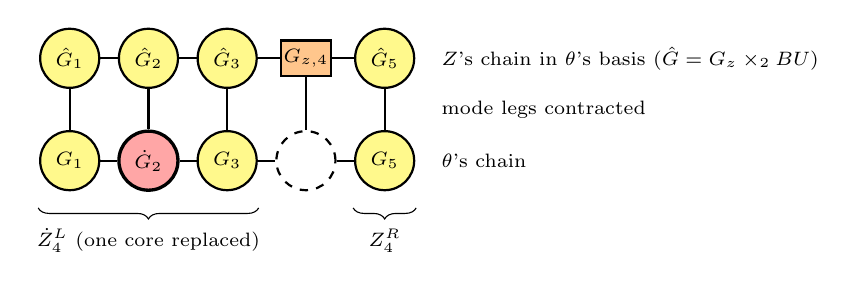
\begin{tikzpicture}[x=10mm,y=10mm]
  \foreach \i in {1,...,5} {
    \ifnum\i=4 \node[holec] (b\i) at (\i,0) {}; \else
      \ifnum\i=2 \node[dotc] (b\i) at (\i,0) {$\dot G_{\i}$}; \else \node[ttc] (b\i) at (\i,0) {$G_{\i}$}; \fi \fi
    \ifnum\i=4 \node[resn] (a\i) at (\i,1.3) {$G_{z,\i}$}; \else \node[ttc] (a\i) at (\i,1.3) {$\hat G_{\i}$}; \fi
    \draw[bnd] (a\i)--(b\i);
  }
  \foreach \i in {1,...,4} { \pgfmathtruncatemacro\j{\i+1} \draw[bnd] (a\i)--(a\j); \draw[bnd] (b\i)--(b\j); }
  \draw[decorate,decoration={brace,amplitude=4pt,mirror}] (0.6,-0.6)--(3.4,-0.6)
     node[midway,below=4pt,font=\scriptsize]{$\dot Z^L_4$ (one core replaced)};
  \draw[decorate,decoration={brace,amplitude=4pt,mirror}] (4.6,-0.6)--(5.4,-0.6)
     node[midway,below=4pt,font=\scriptsize]{$Z^R_4$};
  \node[font=\scriptsize,anchor=west] at (5.6,1.3) {$Z$'s chain in $\theta$'s basis ($\hat G=G_z\times_2BU$)};
  \node[font=\scriptsize,anchor=west] at (5.6,0) {$\theta$'s chain};
  \node[font=\scriptsize,anchor=west] at (5.6,0.65) {mode legs contracted};
\end{tikzpicture}
\caption{The T3-to-T3 two-hole as a ladder: $Z$'s re-based TT cores on top, $\theta$'s below. The hole at core 4 is
the gradient block; the bottom-left $\dot G_2$ makes $\dot Z^L_4$ one term of the tangent zipper. Core 4's own
top rung is $G_{z,4}$ itself, contracted with $BU_4$ (or $\dot{BU}_4$) on the mode leg.}
\label{fig:t3t3}
\end{figure}

\begin{algorithm}[t]
\caption{The T3-to-T3 two-hole $\K_Z\thh$}
\label{alg:t3t3}
\begin{algorithmic}[1]
\Require $Z=(B_z,G_z)$ (tails squashed); $\th=(U,G)$ ($\mathtt C$); $\thh$ ($\mathtt{K+C}$)
\Ensure $\K_Z\thh$
\State $BU,\hat G,Z^L,Z^R,\mathrm{env}$ by \eqref{eq:t3t3} \Comment{per frame: \code{t3_precompute_inner_product_sweep}}
\State $\dot{BU}_i\gets B_{z,i}\dot U_i^\T$;\ $\dot{\hat G}_i\gets G_{z,i}\times_2\dot{BU}_i$
\State $\dot Z^L\gets$ \code{tt_zipper_tangent_left_to_right}$(\hat G,G,\dot{\hat G},\dot G;Z^L)$;\ $\dot Z^R$ likewise from the right
\State blocks by \eqref{eq:t3t3dot}
\Impl{\code{t3_linalg.t3_inner_product_corewise_hessian[_from_sweep]}, \code{t3_linalg.t3_inner_product_corewise_transpose},
\code{tt_operations.tt_zipper_tangent_left_to_right}, \code{tt_zipper_tangent_right_to_left}; called by
\code{ManifoldGeometryOps.tangential_curvature}; uniform: \code{ut3_linalg.ut3_precompute_inner_product_sweep},
\code{ut3_inner_product_corewise_hessian[_from_sweep]}.}
\end{algorithmic}
\end{algorithm}

\subsection{The uniform masking rule}
\label{sec:masking}

On the uniform (packed) layout a second derivative multiplies a direction's \emph{padding} into real slots: the
masks are load-bearing, not hygiene (an unmasked $\thh$ corrupts the real block by $2.6\times10^3$; F15, F18). Every
uniform \code{corewise_hessian} therefore masks $\th$ \emph{and} $\thh$ with the masks of the \textbf{frame it is
handed} --- \code{frame_data[5]}'s up and left masks (\code{uniform_fitting._frame_theta}), not the kind's
\code{self.masks}, which is a strict superset at TT slack (F23) --- runs the mask-free polymorphic kernel, and
re-masks the output (\code{ut3_sampling._masked_point_and_directions}, \code{_remasked_core_gradient};
\code{ut3_masking.ut3_apply_masks}). ``Garbage'' here means \emph{finite} garbage (NaN leaks through any mask that
multiplies). The uniform lift factors clip each block at its real dimensions; padded singular values are exactly 0.

% =====================================================================================================
\section{Shared (tied) Tucker factors}
\label{sec:shared}

On the shared set (SF-T3, after the SF-ETT format of \cite{MR25}) the point is $\Phi(\mathsf T\th_{sh})$, $\mathsf T$ copying each group's factor to its modes, so
the Hessian is the same formula through a \emph{tied} lift (\code{sharing.fv_tied_lift_factors}). A tied coordinate
$\delta U_i=S_i^\T\dot U_g$ (\texttt{docs/shared\_t3\_math.tex}, Prop.\ ``tied tangent space is a tilted subspace'';
that note writes the factors $N\times n$, so its $C_i=\dot US_i$ is this relation transposed) has one raw
factor direction per group, recovered from all the group's coordinates at once against the stacked
$M_g=[S_{i_1}^\T;\dots;S_{i_k}^\T]$ and its SVD $M_g=U_M\,\mathrm{diag}(s_g)\,V_M^\T$ (the companion
\code{SharedFrameData} that the tied projection already uses):
\begin{equation}
  \label{eq:tied}
  \dot U_g=M_g^{+\eps}\begin{bmatrix}\delta U_{i_1}\\ \vdots\\ \delta U_{i_k}\end{bmatrix}
   =V_Mf_\eps(s_g)U_M^\T[\delta U_{i}]_{i\in g},\qquad
  \Lift^\T:\ [\delta U_i]_{i\in g}=(M_g^{+\eps})^\T\textstyle\sum_{i\in g}Y^U_i,
\end{equation}
the same $\dot U_g$ at every group mode; the adjoint sums the group's copies ($\mathsf T^\T$) before the solve's
adjoint. Singleton modes and every TT slot lift as unshared. The normal part is taken against the \emph{tied}
gradient (the geometry's tied \code{project}), and the outer $\Pi_{sh}$ of \eqref{eq:newton} ties the result.
\begin{itemize}
\item \textbf{$s_g$ replaces the group modes' own spectra.} The tied lift inverts $M_g$, never a group mode's
  $S_i^\T$, which can be rank-deficient at a perfectly regular shared point (a group rank above a member's ceiling
  $r_{i-1}r_i$). So \code{lift_sigma_min} $=\min(\sigma(T_i),\ \sigma(S_i)$ for untied $i$, $s_g)$
  (\code{geometry._lift_sigma_min}). A per-mode lift represents the same tangent but not a tied direction; its
  quadratic form is off by $5.6$--$19$ at such points (the tests use these \emph{group-ceiling} structures).
\item \textbf{Padded restarts.} A zero-padded shared restart's new $s_g$ levels are zero and filter to exactly 0:
  the gated tied channel gets no curvature, as it gets no first-order motion; the TT slots carry the escape. On the
  uniform layout the group filter is additionally zeroed on the padded $s_g$ levels by the frame's group rank
  mask and clipped at the group's real dimensions (\code{ufv_operations.ufv_tied_lift_factors}).
\item The shared \emph{corewise} geometry needs no lift: its exact Hessian is the per-group mean (its tied
  \code{project}) of the plain one. The shared retraction's second order is measured (F14), not proven.
\end{itemize}

\begin{algorithm}[t]
\caption{The tied lift and its adjoint (one nontrivial group $g$)}
\label{alg:tied}
\begin{algorithmic}[1]
\Require companion $(U_M,s_g,V_M,\text{row splits})$ of $M_g$; $\eps$; coordinates $[\delta U_i]_{i\in g}$, or raw $[Y^U_i]_{i\in g}$
\State $f\gets f_\eps(s_g)$, clip $\mathrm{rcond}=\mathrm{dtype}\,\eps\cdot\max(\sum_{i\in g}n^D_i,n_g)$ \Comment{\code{_tied_filter}}
\State lift: $\dot U_g\gets V_M\,\mathrm{diag}(f)\,U_M^\T\,[\delta U_i]_{i\in g}$; $\dot U_i\gets\dot U_g$ for $i\in g$ \Comment{\code{_tied_filtered_solve}}
\State adjoint: $Y_g\gets\sum_{i\in g}Y^U_i$;\ $[\delta U_i]\gets U_M\,\mathrm{diag}(f)\,V_M^\T Y_g$, split by rows \Comment{its transpose}
\Impl{\code{sharing.fv_tied_lift_factors} (fills \code{LiftFactors.shared_data}, \code{tied_filters}),
\code{sharing._tied_filter}, \code{_tied_filtered_solve[_transpose]} (with \code{eps=None} bit-identical to the
tied projection's solve), dispatched inside \code{tv_corewise_lift[_transpose]}; uniform:
\code{ufv_operations.ufv_tied_lift_factors}.}
\end{algorithmic}
\end{algorithm}

% =====================================================================================================
\section{The canonical zero-point frame and the Newton reference}
\label{sec:zero}

The default Newton reference (\code{g0_reference='zero'} on the manifolds) is $\|\Pi\Jac^\T(\omega^2\odot r_0)\|$,
$r_0=A\cdot0-y$, at the zero tensor of $x_0$'s ranks: the relative stop $\|g\|\le\texttt{gtol\_rel}\cdot\|g_0\|$
and the forcing term $\eta=\min(\frac12,(\|g\|/\|g_0\|)^{\texttt{cg\_forcing\_power}})$ are measured against it.
At $X=0$ every orthonormal completion is a valid frame and the gradient norm depends on the choice, so the library
fixes one (I-29):

\begin{algorithm}[h]
\caption{The canonical zero-point frame}
\label{alg:zero}
\begin{algorithmic}[1]
\Require a frame's \emph{structure} (core shapes; unstacked); sharing groups (singletons their own); seed $=0$
\For{each group $g$ with key $k_g=\min g$}
  \State $G\gets$ \code{RandomState([seed, k_g]).standard_normal((n_g, N_g))} \Comment{keyed legacy stream}
  \State $Q,R\gets\mathrm{qr}(G^\T)$ (reduced);\ $U_g\gets(Q\,\mathrm{sign}(\mathrm{diag}R))^\T$, replicated over $g$ \Comment{sign-fixed Haar rows}
\EndFor
\State $O_i,P_i,Q_i\gets$ identity prefixes (orthonormal), $P_d=0$, $Q_1=0$ \Comment{base point $=0$}
\Impl{\code{fv_operations.fv_zero_point_frame} (\code{_haar_rows}, \code{_identity_prefix}, \code{ZERO_FRAME_SEED});
uniform \code{ufv_operations.ufv_zero_point_frame} (unpack, build, pack); geometry member \code{zero_point_frame};
the reference: \code{optimizers._resolve_g0_reference}, \code{_zero_reference_gnorm}.}
\end{algorithmic}
\end{algorithm}

Three properties hold by construction: \emph{rank independence} (each group draws from its own keyed stream, so a
factor never depends on another mode's rank or size --- bit-identical); \emph{nesting} (QR column $j$ depends only on
draw rows $\le j$, so level $r$'s factor is exactly the leading-row prefix of level $r{+}1$'s, and the references
along a continuation ladder are taken on nested subspaces); \emph{layer independence} (the uniform twin builds the
same real blocks, $\le3.9\times10^{-16}$; the 44 ragged/uniform optimizer pairs agree to $3.5\times10^{-12}$, F37).
Haar only for $U$: the Tucker factor is the only part of the frame that meets the data, and any
coordinate-aligned completion gives a reference of exactly 0 on data with no energy on the leading coordinates
(F32; Haar seeds 0--5 gave 9.5--24 there). The reference is a \emph{convention} --- a deterministic data-gradient
scale at these ranks, good to an $O(1)$ factor (another seed or a mode rotation moved it by up to $\sim1.7\times$) ---
harmless for a relative stop. The corewise geometries have none (zero cores are a critical point): their default is
the warm start. A vanishing zero reference falls back to the warm start with a warning (default) or raises (explicit).

% =====================================================================================================
\section{The trust region}
\label{sec:tr}

The exact Hessian is indefinite away from a minimizer, so \code{hessian='exact'} defaults to
\code{step_control='trust_region'}: Steihaug--Toint CG \cite{Ste83,NW06} inside $\|p\|\le\Delta$ and one trial
retraction, accepted on the ratio $\rho$ of actual to predicted change. This is what makes the exact model's $\rho$
meaningful: with a second-order retraction the predicted and actual changes agree to $O(\|p\|^3)$.

\paragraph{One CG body for both step controls} (\code{_cg_body}, I-5). The state carries the radius and a
boundary flag; every branch is an \code{xnp.where}, so the same body drives the eager loop and
\code{lax.while_loop}. With $\alpha=r^\T r/d^\T\Hop d$: if $d^\T\Hop d>0$ and $\|p+\alpha d\|\le\Delta$ it is a plain
CG step; if $\|p+\alpha d\|>\Delta$, or $d^\T\Hop d\le0$ with $\Delta$ finite, it steps to the boundary,
\begin{equation}
  \label{eq:tau}
  p\gets p+\tau d,\qquad \tau=\frac{-p^\T d+\sqrt{(p^\T d)^2+\|d\|^2(\Delta^2-\|p\|^2)}}{\|d\|^2}\ \ (\|p+\tau d\|=\Delta,\ \tau\ge0),
\end{equation}
and stops. With $\Delta=\infty$ (line search) nonpositive curvature takes a zero step and stops: the
pre-trust-region truncated CG, bit for bit on eager numpy. No $\infty$ ever enters arithmetic.

\begin{algorithm}[t]
\caption{Newton--CG with the trust region (one row per trial)}
\label{alg:tr}
\begin{algorithmic}[1]
\Require $x_0$; references $\|g_0\|$ (Section~\ref{sec:zero}); forcing power $\kappa$ (default $\frac12$; $1$ for a q-quadratic tail)
\State build the local model at $x$; $g$, $f$ \Comment{\code{Problem.local_model(hessian='exact')}}
\Loop
  \If{$\|g\|\le\texttt{gtol\_rel}\,\|g_0\|$} \Return $x$ (\code{'gradient'}) \EndIf
  \State $\eta\gets\min(\frac12,(\|g\|/\|g_0\|_{cg})^\kappa)$ \Comment{forcing term}
  \State first step: $\Delta_0\gets\|g\|^3/g^\T\Hop_{GN}g$ (or $\|g\|$), $\Delta_{\max}\gets10^4\Delta_0$ \Comment{\code{_initial_radius}}
  \State $p\gets$ Steihaug CG on $\Hop p=-g$ to $\eta\|g\|$ inside $\Delta$ \Comment{\code{_cg_solve}}
  \State if $g^\T p\ge0$: $p\gets-g\min(1,\Delta/\|g\|)$ (a boundary step if scaled)
  \State $\mathrm{pred}\gets g^\T p+\frac12(p^\T\Hop_{GN}p+p^\T\Lift^\T\K_N\Lift p)$ \Comment{one two-hole}
  \State $\rho\gets(f(R_x(p))-f)/\mathrm{pred}$ if $\mathrm{pred}<0$, else NaN
  \State \textbf{if} $\rho<\frac14$ or NaN: $\Delta\gets\frac14\|p\|$;\ \textbf{elif} $\rho>\frac34$ and boundary: $\Delta\gets\min(2\Delta,\Delta_{\max})$
  \If{$\rho>0.1$} accept: $x\gets R_x(p)$, rebuild the model
  \Else \ keep $x$ and its model
    \State \textbf{stop} \code{'objective_floor'} if $|\mathrm{pred}|\le10\,\epsilon_{\mathrm{res}}(\|\omega\odot y\|\,\|\omega\odot r\|+|f|)$
    \State \textbf{stop} \code{'trust_region_floor'} if $\Delta<10^{-12}\Delta_0$ (checked second)
  \EndIf
\EndLoop
\Impl{\code{optimizers.newton_cg}; CG \code{_cg_solve}, \code{_cg_core}, \code{_cg_body}; \code{LocalModel.gn_quadratic},
\code{curvature_quadratic} (constants \code{_TR_ACCEPT}, \code{_TR_SHRINK_BELOW}, \code{_TR_SHRINK},
\code{_TR_EXPAND_ABOVE}, \code{_TR_EXPAND}, \code{_TR_RADIUS_MAX_REL}, \code{_TR_RESOLUTION_FACTOR},
\code{_TR_RADIUS_FLOOR_REL}); $\epsilon_{\mathrm{res}}$ = \code{_resolution_eps} (host-side, dtype-only); per-row
\code{NewtonInfo}.}
\end{algorithmic}
\end{algorithm}

\paragraph{The floors.} They are checked only after a \emph{rejection} (an accepted step never stops the run).
$\epsilon_{\mathrm{res}}=\max$ \code{np.finfo(dtype).eps} over the residual's floating leaves, read from dtypes
only (no device sync), so a float32 fit is judged at float32's resolution. \code{'objective_floor'} is not a
failure: the model change is below the objective's floating-point resolution, so the attainable accuracy is
reached. A rejected trial keeps $x$ and its local model and emits its own history row; $\Delta_0$ is the
Gauss--Newton Cauchy length whatever the Hessian. Measured (seeded probe-derivative restart, F19): Gauss--Newton
with Armijo 39 steps / 130 Hessian-applies, exact with the trust region 8 / 23 at power 1.0, 10 / 28 at 0.5,
0 rejected; the q-quadratic tail $e_{k+1}\le0.92\,e_k^2$ at power 1.0 (F22).

% =====================================================================================================
\section{Verification}
\label{sec:verify}

Every displayed identity was checked against the library at \texttt{f739085} by a scratch script (numpy float64;
jax float64 for the Lagrangian; complex-step derivatives, which are exact, for the two-holes); Table~\ref{tab:checks}
lists the relative residuals.
\begin{table}[t]
\centering
\small
\begin{tabular}{@{}l p{0.68\textwidth} r@{}}
\toprule
& check & residual \\
\midrule
C1 & \eqref{eq:factors}: $H_i=O_i\times_2S_i^\T$; $P_{>i}=T_iQ_{>i}$; spectra; $\|X\|^2=\|S_1^\T\|_F^2$ & $\le8.4{\times}10^{-16}$\\
C2 & Prop.~\ref{prop:lift}: $D\Phi[\Lift v]=\Emap v$ on minimal / Tucker-slack / TT-slack frames & $\le2.4{\times}10^{-15}$\\
C3--4 & $\Lift_\eps^\T$ is the adjoint at $\eps=10^{-2}\|X\|$; $\max f_\eps=1/(2\eps)$; $M^{+\eps}=(M^\T M+\eps^2I)^{-1}M^\T$ & $\le1.9{\times}10^{-15}$\\
C5 & $\grad f=P_X\nabla f$; $N$ is normal & $\le9.9{\times}10^{-16}$\\
C6 & $\ip{N}{D^2\Phi[\thh,\thh']}=\ip{\thh'}{\K_N\thh}$ (dense double replacement); a vertical $\thh_v$ has
  $\K_N\thh_v=0$ and does not change the form, while $\|\K_{A^\T r}\thh_v\|\approx10^4$ & $\le1.2{\times}10^{-13}$\\
C7 & \eqref{eq:newton} $=\Pi\Lift^\T\nabla^2_\th\Lambda\Lift\Pi$ (\code{jax.jvp} of \code{jax.grad}); $\nabla_\th\Lambda=0$;
  level 1 $=\Pi\Lift^\T\nabla^2_\th(f\circ\Phi)\Lift\Pi$ & $\le4.5{\times}10^{-14}$\\
C8 & $\ip{p}{\Hop p}$ vs $\frac{d^2}{dt^2}f(R(tp))$ (Richardson; level 2) / vs $\frac{d^2}{dt^2}f(\Phi(\th+t\Lift p))$ (level 1) & $3.7{\times}10^{-6}$ / $2.5{\times}10^{-10}$\\
C9 & the two-holes (probe derivatives, apply derivatives, T3--T3) $=$ complex-step $d/ds$ of their one-holes; the
  block sum \eqref{eq:blocksum}; symmetry; order 0 $=$ plain probe & $\le4.6{\times}10^{-16}$\\
C10 & the written recurrences $\dot\mu$, \eqref{eq:tautilde}, \eqref{eq:tautildedot}, $\dot{\dxt}$ vs the kernels & $\le4.3{\times}10^{-16}$\\
C11 & the factored assemblies \eqref{eq:pairs}, \eqref{eq:asmjetdot} $=$ the nine-term binomial product rule & $\le6.3{\times}10^{-16}$\\
C12 & tied lift \eqref{eq:tied}: $D\Phi[\Lift v]=\Emap v$ at a group-ceiling point; $=M_g^+[\delta U_i]$; adjoint & $\le5.1{\times}10^{-16}$\\
C13 & zero frame: nested, rank-independent, base point 0, the recipe by hand (orthonormal to $6.7{\times}10^{-16}$) & $0$\\
C14 & $\Hop=$ GN $+$ \code{curvature_hvp}; quadratic split; exact gradient $\equiv$ GN gradient; default $\eps$ & $\le4.4{\times}10^{-16}$\\
\bottomrule
\end{tabular}
\caption{The equation checks (scratch script against \texttt{f739085}; relative residuals).}
\label{tab:checks}
\end{table}
At C8 the point was far from a minimizer: the exact quadratic form was $-5449.96$ against the Gauss--Newton $30.33$,
the retraction difference quotient $-5449.94$. The living guarantees are \code{tests/backend/test_curvature.py},
\code{tests/backend/test_uniform_curvature.py}, the exact oracle sweep (720 always-on cases, max
$2.5\times10^{-14}$; 8000 slow-tier cases, max $2.6\times10^{-11}$) and the dispatch tests' \code{TestCurvatureJvpOracle}
(\code{jax.jvp} of each one-hole, $\le10^{-12}$). A frontend finite-difference check of the Hessian
(\code{MANIFOLD.norm(H_fd - hessian(p))}) passes the safe-mode gauge check, which is scaled by the operands
(\code{tv_gauge_residual(frame, variations, scale)}, I-38). Measurements:
\code{docs/contributor/verification_records.md}; design record: \code{docs/contributor/curvature_internals.md}.

\paragraph{Costs.} An exact Hessian-apply costs $2.8$--$3.9\times$ a Gauss--Newton one (numpy CPU, six kinds), with a
memory peak about twice the GN transpose's; the uniform exact CG compiles once per run.

\begin{small}
\begin{thebibliography}{9}
\setlength{\itemsep}{1pt}
\bibitem{T4S} N.~Alger, B.~Christierson, P.~Chen, O.~Ghattas, \emph{Tucker Tensor Train Taylor Series},
  arXiv:2603.21141 (2026); App.~A for the frame, gauge, tangent space and T3-SVD; \S6 for probing.
\bibitem{AMT13} P.-A.~Absil, R.~Mahony, J.~Trumpf, \emph{An extrinsic look at the Riemannian Hessian}, GSI 2013.
\bibitem{PB20} M.~Psenka, N.~Boumal, \emph{Second-order optimization for tensors with fixed tensor-train rank},
  arXiv:2011.13395 (2020) --- the TT Weingarten map with $R_k^{-1}$, the analogue of $T_i^{+}$.
\bibitem{NRO22} A.~Novikov, M.~Rakhuba, I.~Oseledets, \emph{Automatic differentiation for Riemannian optimization on
  low-rank matrix and tensor-train manifolds}, SIAM J.\ Sci.\ Comput.\ 44(2), 2022 (arXiv:2103.14974).
\bibitem{MR25} A.~Molozhavenko, M.~Rakhuba, \emph{Optimization on the extended tensor-train manifold with shared
  factors}, Comput.\ Appl.\ Math.\ 45:221 (2026); arXiv:2508.20928 (2025).
\bibitem{AM12} P.-A.~Absil, J.~Malick, \emph{Projection-like retractions on matrix manifolds}, SIAM J.\ Optim.\
  22(1), 2012.
\bibitem{Ste83} T.~Steihaug, \emph{The conjugate gradient method and trust regions in large scale optimization},
  SIAM J.\ Numer.\ Anal.\ 20(3), 1983.
\bibitem{NW06} J.~Nocedal, S.~Wright, \emph{Numerical Optimization}, 2nd ed., Springer 2006, Alg.~4.1 and 7.2.
\end{thebibliography}
\end{small}

\end{document}
